% Aaron's poster for the Earlham Annual Research Conference
%
% Template based on PetaKit "how" poster
%
\documentclass[a0]{a0poster}

%
\pagestyle{empty}
%
\setcounter{secnumdepth}{0}
\newcommand{\standardsize}{\fontsize{28}{33}\selectfont}

% The textpos package is necessary to position textblocks at arbitary 
% places on the page.
%
\usepackage[absolute]{textpos}
\usepackage{url}

% Graphics to include graphics. Times is nice on posters, but you
% might want to switch it off and go for CMR fonts.
%
\usepackage{graphicx,wrapfig,times}

% Avoid unnecessary hyphenation in paragraphs. Also requires
% \raggedright below, after \begin{document}.
%
\usepackage[none]{hyphenat}

% These colours are tried and tested for titles and headers. Don't
% over use color!
%
\usepackage{color}
\definecolor{DarkBlue}{rgb}{0.1,0.1,0.5}
\definecolor{Red}{rgb}{0.9,0.0,0.1}
\definecolor{Green}{rgb}{0.0,0.6,0.1}

% See documentation for a0poster class for the size options here
%
\let
\Textsize
\normalsize
\def\Head#1{\noindent\hbox to \hsize{\hfil{\LARGE\color{DarkBlue} #1}}\bigskip}
\def\LHead#1{\noindent{\LARGE\color{DarkBlue} #1}\bigskip}
\def\Subhead#1{\noindent{\large\color{DarkBlue} #1}}
\def\Title#1{\noindent{\VeryHuge\color{Green} #1}}

% Set up the grid
%
% Note that [40mm,40mm] is the margin round the edge of the page --
% it is _not_ the grid size. That is always defined as 
% PAGE_WIDTH/HGRID and PAGE_HEIGHT/VGRID. In this case we use
% 23 x 12. This gives us three columns of width 7 boxes, with a gap of
% width 1 in between them. 12 vertical boxes is a good number to work
% with.
%
% Note however that texblocks can be positioned fractionally as well,
% so really any convenient grid size can be used.
%
\TPGrid[40mm,40mm]{23}{12}      % 3 cols of width 7, plus 2 gaps width 1

\parindent=0pt
\parskip=0.5
\baselineskip

\begin{document}
\large
\raggedright

% Understanding textblocks is the key to being able to do a poster in
% LaTeX. In
%
%    \begin{textblock}{wid}(x,y)
%    ...
%    \end{textblock}
%
% the first argument gives the block width in units of the grid
% cells specified above in \TPGrid; the second gives the (x,y)
% position on the grid, with the y axis pointing down.
%
% You will have to do a lot of previewing to get everything in the 
% right place.
%
% Watch out for hyphenation in titles - LaTeX will do it
% but it looks awful.
%

% Title
%
\begin{textblock}{23}(0,0)
\Title{\textit{Computer City: Sewers}: An Educational Game to Teach Digital Logic}
\end{textblock}

% Authors and institutions
%
\begin{textblock}{20}(0,0.6)
\LHead{Aaron Weeden}
\hfil
\break
\textsl{Earlham College -- amweeden06@earlham.edu}
\end{textblock}

% Abstract
% 
%\begin{textblock}{23}(0,1.2)
%\large
%\input{abstract.tex}
%\normalsize
%\end{textblock}

% Logos at top of each column.
% 
%\begin{textblock}{2}(2.2,3.2)
%\includegraphics{../artwork/littlefe.eps}
%\end{textblock}
%
%\begin{textblock}{2}(10.9,3.1)
%\includegraphics{../artwork/bccd.eps}
%\end{textblock}
%
%\begin{textblock}{2}(18.0,3.4)
%\includegraphics{../artwork/cserd.eps}
%\end{textblock}

% First column 
% 
\begin{textblock}{6}(0,2.6)
\hrule
\medskip
\LHead{Background}
\standardsize
Since 2000, there has been a general decrease in enrollment and retention of students in computer science departments across the country \citep{Sung}, \citep{Wu}, \citep{Leutenegger}.  The diversity of participants in these departments has also been shown to decrease in upper-level courses, with fewer minorities and women participating in these classes \citep{Sung}, \citep{Wu}.  One of the more promising solutions to these problems is the incorporation of computer games into the computer science curriculum.  Games have been shown on multiple occasions to have a positive effect on motivation and engagement of students; and with the inclusion of educational components, they also provide increases in learning \citep{Wu}, \citep{deLaet}, \citep{Bayliss}, \citep{Wolz}, \citep{Flavor}, \citep{Belfore}.  With this in mind, the author of this poster has developed \textit{Computer City:  Sewers}, an educational game to teach digital logic, a fundamental topic in computer science.
\end{textblock}

\begin{textblock}{11}(0,2.7)
\begin{center}
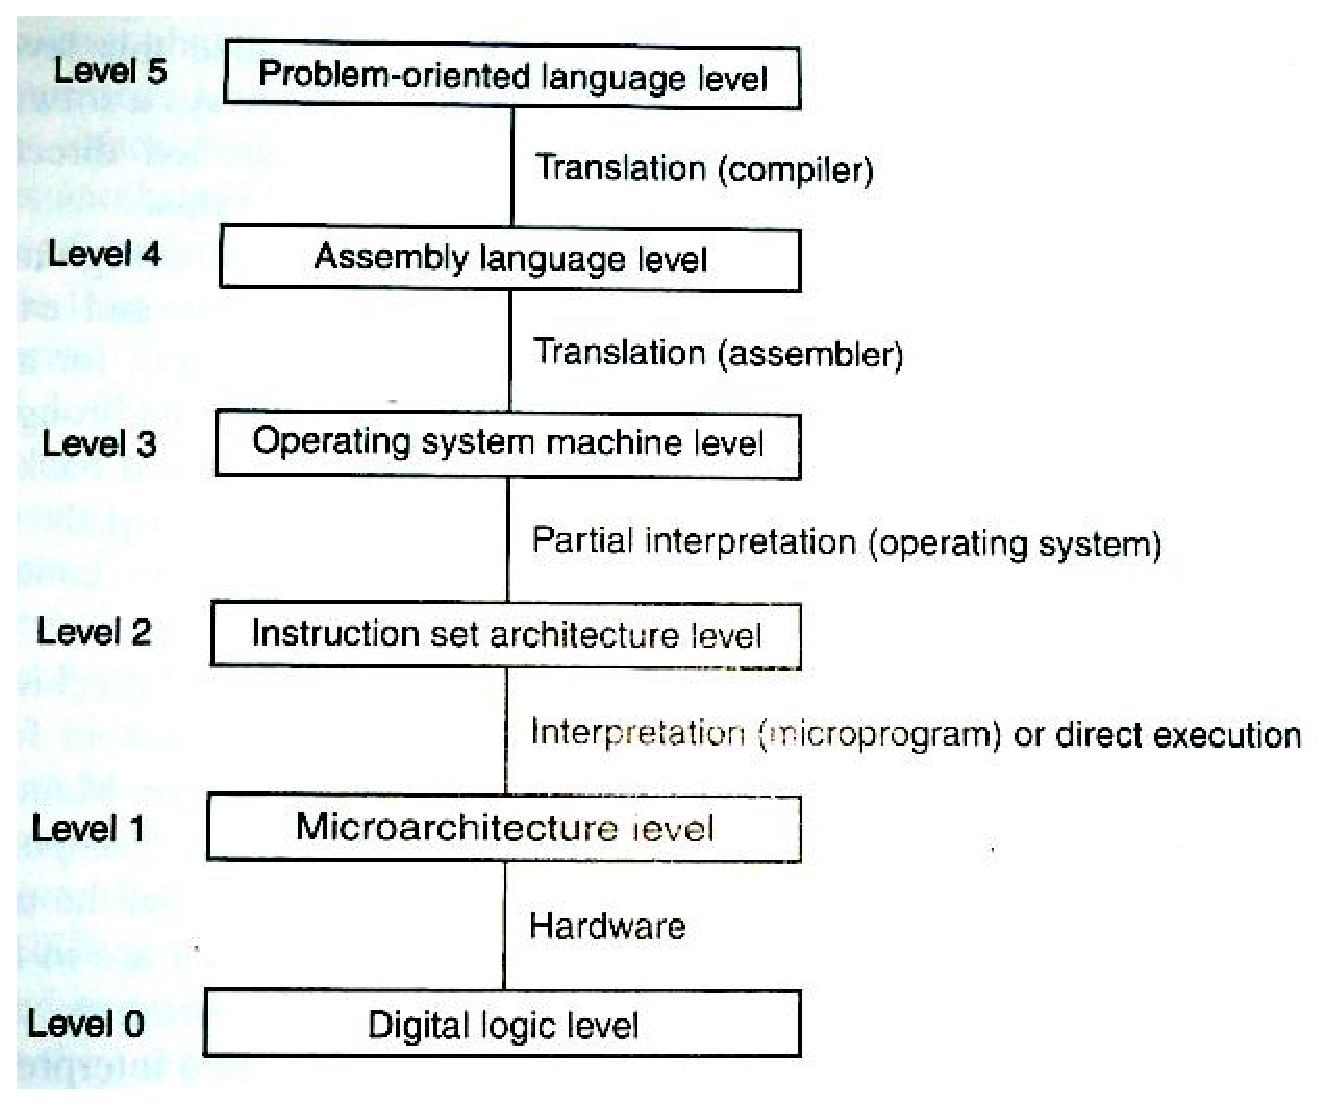
\includegraphics[scale=2.4]{Hierarchy.eps}
Figure 1:  Tanenbaum's Hierarchy
\end{center}
\end{textblock}

\begin{textblock}{11}(0,2.7)
\begin{center}
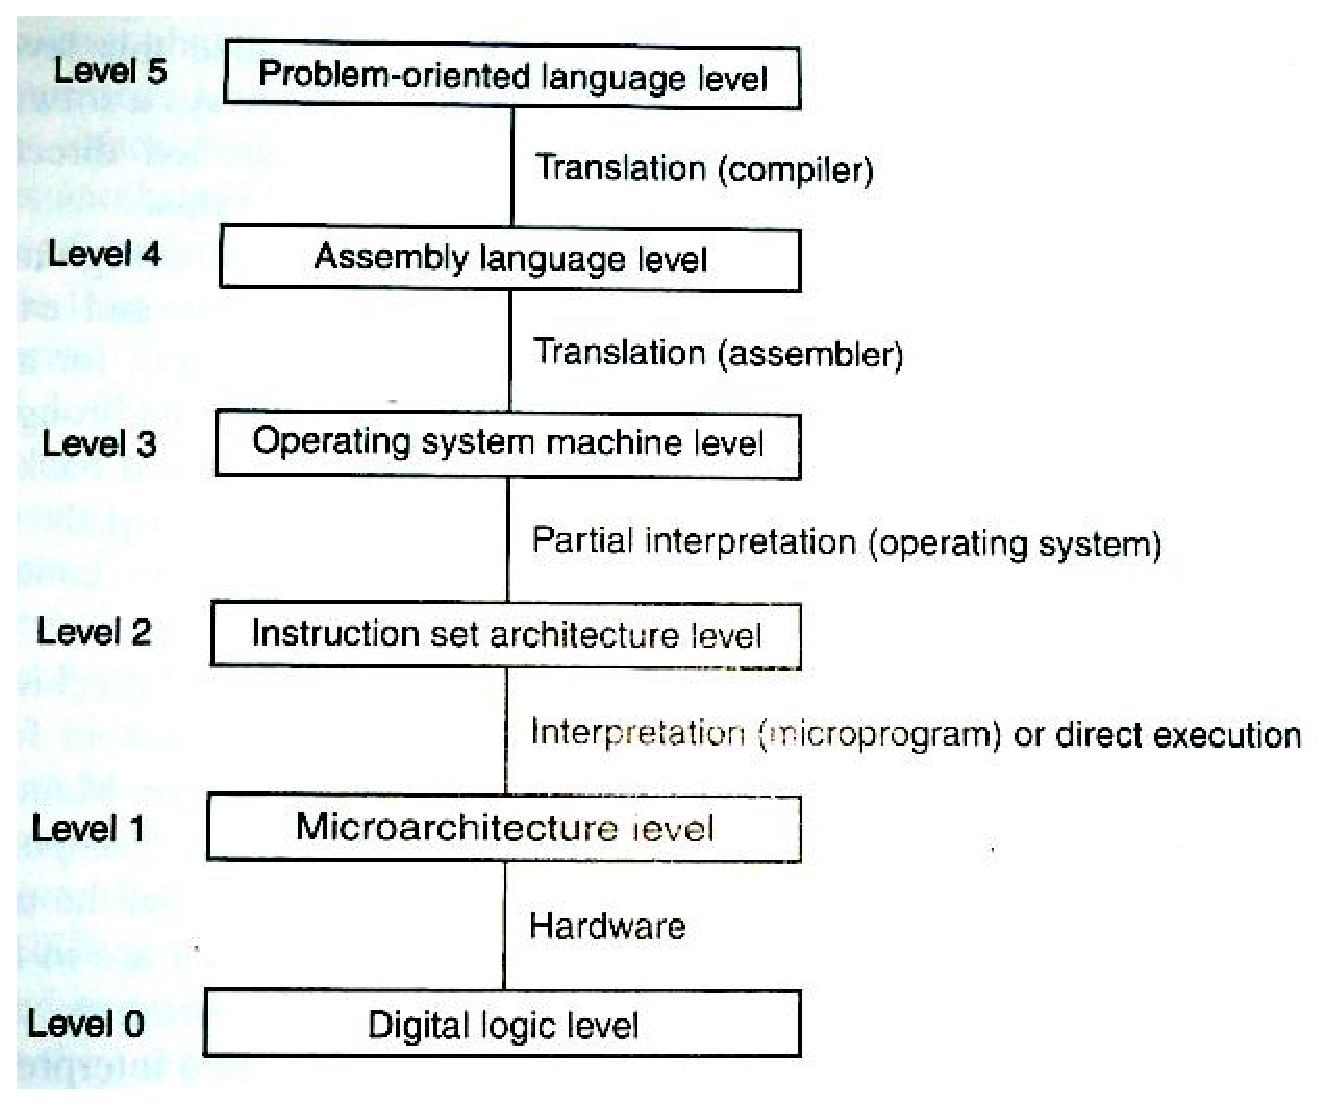
\includegraphics[scale=2.4]{Hierarchy.eps}
Figure 2:  The NAND gate and its truth table
\end{center}
\end{textblock}

\begin{textblock}{6}(0,2.6)
\hrule
\medskip
\LHead{Digital Logic}
\standardsize
The computer architecture can be thought of as a hierarchy, as seen in Figure 1 \citep{Tanenbaum}.  Programmers and other humans interact with the higher levels of the hierarchy, while the machine itself interacts with the lower levels.  Digital logic is the foundation of this hierarchy.  At this level, logic and arithmetic are performed on binary values (zeros and ones).  Conceptually, this logic and arithmetic can be explained by gates and truth tables.  Gates are objects that take input values and produce an output value.  Truth tables list the possible combinations of inputs and the outputs of those combinations.  The basic gate, the NAND gate (Figure 2), creates the foundation of the entire computer architecture; every other gate can be built as combinations of NANDs, and any functionality of the computer architecture at higher levels can be broken down into functionality of NAND gates at the digital logic level.
\end{textblock}

\begin{textblock}{6}(0,2.6)
\hrule
\medskip
\LHead{Storyline}
\standardsize
\textit{Computer City: Sewers} presents a hypothetical city as a metaphor for the computer architecture.  In such a city, every aspect of the computer architecture has a corresponding metaphor; buses in a computer correspond to the bus system of the city, addresses in computer memory correspond to the addresses of buildings in the city, and so forth.  The playable portion of the city is the sewer, conceptually the lowest level of the city, corresponding to digital logic, conceptually the lowest level of the computer hierarchy.  The player takes the role of Bitty, who has been placed underground by his/her superiors to assist the engineers who work in the sewers.  Engineers require logic gates to do their work, but they do not have the means to produce them and are not aware of the effects of their work.  The work done by the engineers affects the higher levels of the city, but these effects are hidden from the engineers and Bitty.  To provide gates for the engineers, Bitty consults with a manufacturer, who is able to produce gates if Bitty is able to construct blueprints for them.
\end{textblock}

% Second column 
% 
\begin{textblock}{6}(6,2.6)
\hrule
\medskip
\LHead{Gameplay}
\standardsize
The player uses the keyboard to move Bitty around and talk to other characters.  A Heads-Up Display (HUD) at the bottom of the screen allows the player to see current game statistics, save, load, and quit.  The gate and truth table corresponding to the current player task are also displayed on the HUD.
The player is assigned tasks by interacting with engineers.  Each engineer asks Bitty to return with a gate meeting certain specifications:  given certain inputs the gate should produce certain outputs.  To accept the task, the player must complete a truth table based on the engineer's description of the gate's specifications.  
To construct a gate, Bitty consults with a manufacturer, who is able to construct gates for which there are existing blueprints.  The manufacturer initially knows only how to build a NAND gate, but each time the player constructs a new blueprint the manufacturer is able to build a new gate, which the player can use in subsequent blueprints.  Thus, gates are constructed from other gates.
\end{textblock}

\begin{textblock}{11}(6,2.7)
\begin{center}
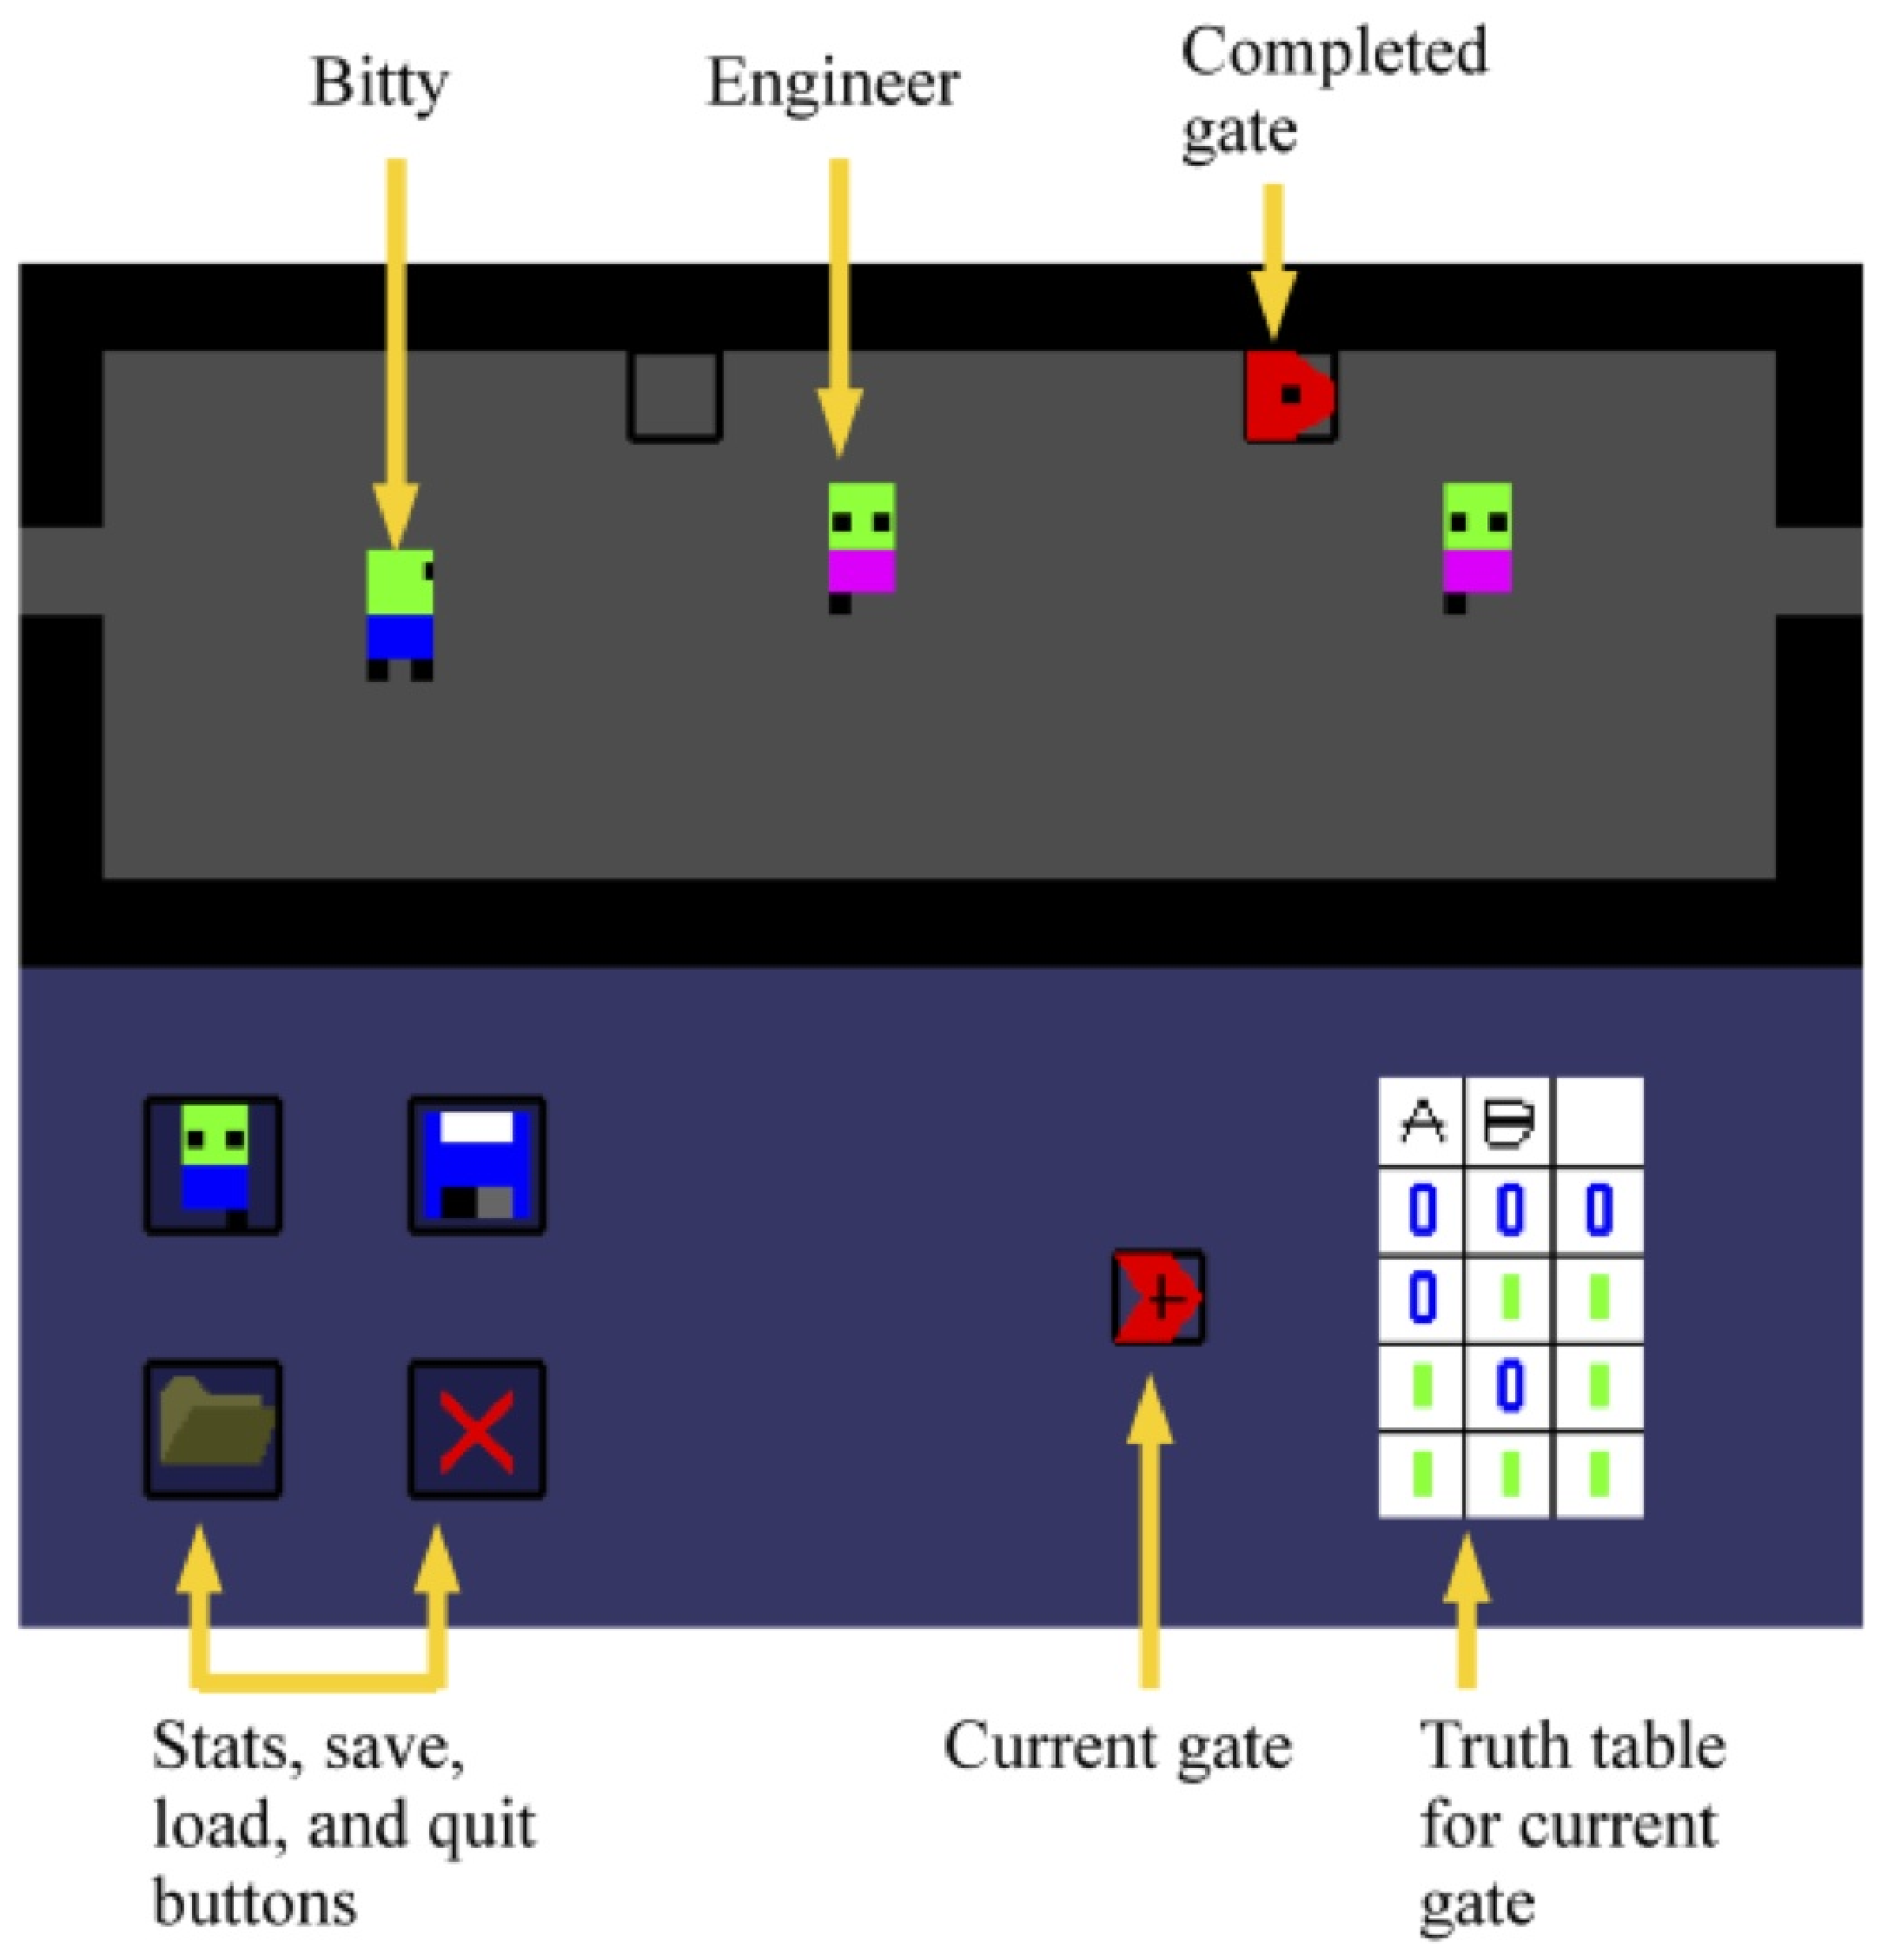
\includegraphics[scale=2.4]{ScreenShot.eps}

A gameplay screenshot
\end{center}
\end{textblock}

% Third column 
% 
\begin{textblock}{6}(6,2.6)
\hrule
\medskip
\LHead{Learning Goals}
\standardsize
{\textit{Computer City:  Sewers} hopes to teach the following skills and concepts:
Basic Gate Recognition (NAND, NOR, NOT, AND, OR, XOR)
Truth Table Construction
Abstraction -- Complex gates are built from collections of simpler gates
Information Hiding -- Lowers levels construct a framework but are unaware how the framework is used, and upper levels use the framework but are unaware how it is constructed.
\end{textblock}

\begin{textblock}{5.5}(17,2.6)
\hrule
\standardsize
\medskip
\LHead{Design Strategies}
These strategies were obtained from research on the common design practices of educational computer game developers.  They include:
Game centered on the lesson -- The player should be unable to progress through the game without using the knowledge gained from the game's underlying lesson.
Clear connections to real-world applications -- Objects in the game should closely resemble their real-world counterparts, and the vocabulary of the game should closely match that of the real world.
Decision-making opportunities -- Giving the player choices encourages exploration, which increases both motivation and the amount of material learned.
Constant feedback -- When the player makes a decision, he/she should be aware of the results immediately.  In this way, the player is able to understand the connection between decisions and their consequences.  
\end{textblock}

\begin{textblock}{5.5}(17,2.6)
\hrule
\standardsize
\medskip
\LHead{Goals for the Future}
Playtesting study -- An empirical study of the game's effectiveness in learning outcomes
New levels -- The player learns about the microarchitecture level and its connection to the digital logic level
Classroom use -- Does the game fit well within a university-level curriculum?
  
\end{textblock}

\begin{textblock}{5.5}(17,2.6)
\hrule
\standardsize
\medskip
\LHead{References}
\input{references.tex}  
\end{textblock}

\end{document}
